\section{Technical Developments}

%%%%%%%%%%%%%%%%%%%%
\subsection{Testing}
%%%%%%%%%%%%%%%%%%%%
To test the poker server, and ensure that the gameplay is correct, the
Haskell testing framework QuickCheck\parencite{claessen2000} was used. This
framework uses automated testing of functions using random input data to
verify properties. For example, suppose we want to test the function which
prompts the user for an amount to bed, then makes that bet. We can define a
few properties which should hold when this occurs.
Firstly, the amount of money present in the system should remain the same.

\begin{lstlisting}[label={code:moneypreserved}, caption=An example QuickCheck property]
prop_BetMoneyPreserved player pot =
    let (newPlayer, newPot) = bet player pot
    player.money + pot.money == newPlayer.money + newPot.money
\end{lstlisting}

We can then run the QuickCheck property displayed in Listing~\ref{code:moneypreserved}
and provided our types can have a random instance determined for them, it
will feed in these random inputs to our function and check that the property
holds true. If the property is proved false, the checker will print out the
inputs that caused the failure, allowing the faulty code to be easily triggered
and traced back.

In this way, we can easily build up a large amount of simple tests to confirm
that the base assertions hold true. We can then rerun these tests automatically
on every code change, to confirm that we have not broken any expected
behaviour. In this way, as long as the assertions are correct, our whole
system should be robust.

Upon these base assertions we can then extrapolate to a much larger scale.
If the balance of the system is retained in the few functions that touch
the balance, it is clear the the balance during a whole game will be maintained.

One downside of this system arises when a large portion of the codebase is
impure, and has to interact with a network, a database, or other impure code.
The QuickCheck library cannot automatically define random instances for
networks or databases (as there is no obvious sane way to do so), and so we
would have to manually define a large mockup system to simulate a database
and a network connection.

To resolve these issues, another way of testing the system is black box
testing, which we can semi automate using the developed AI's. A user only
has a very few select inputs they can make, and at any point in the game,
a user can only make an input that is valid for the users current situation.
For example, they cannot ``Call'' if they do not have enough chips to do so.
In this way, regardless of the data the user sends us, they cannot perform
an invalid action, so all we need to determine is that any sequence of valid
actions is itself a valid action. By running the server and letting AI's
connect to it, and play each other, we can very quickly test large amounts
of different actions in sequence. This method has helped uncover some rare
crashes in the system.

In practice, a mixture of the two testing methods is most effective. By
creating larger impure functions out of small, testable pure functions, we
can ensure that our primitive building blocks are valid, and then use automated
block box testing to hit some of the rarer code paths and ensure that they
too are valid.

%%%%%%%%%%%%%%%%%%%%%%%%%%%%%%%%
\subsection{Experimental Design}
%%%%%%%%%%%%%%%%%%%%%%%%%%%%%%%%
To test out the effects of the shuffle algorithms and random sources, multiple
testing programs have been created. The first method is a simple shuffle
tester. A shuffle method is chosen, along with a source of randomness. Then,
multiple hands are dealt using the selected shuffle and random source, and
the cards picked are recorded, and displayed in a graph format.

\begin{figure}[h]
    \frame{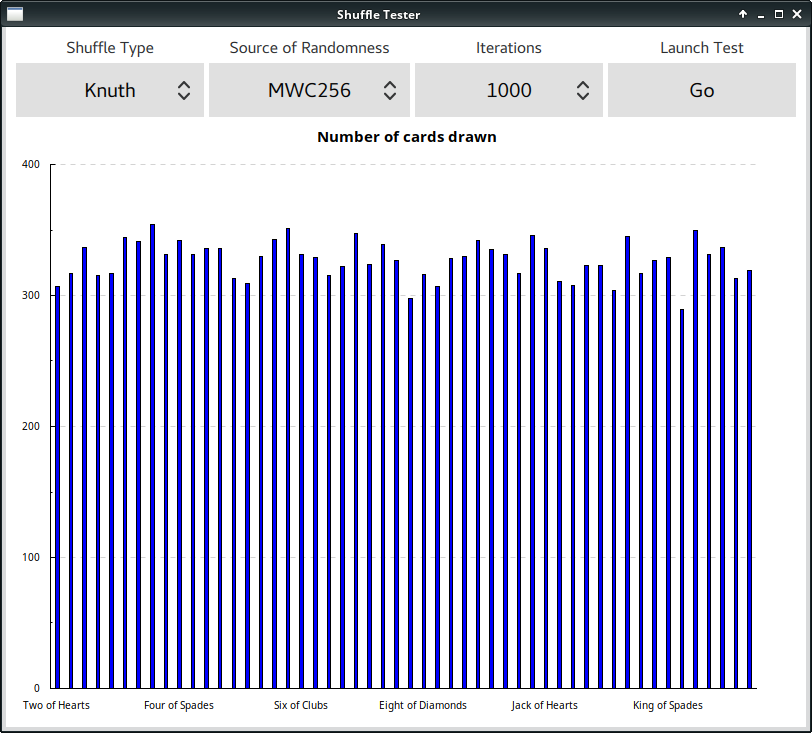
\includegraphics[width=\linewidth]{../images/shuffletester.png}}
    \caption{The shuffle tester program}%
    \label{fig:shuffletester}
\end{figure}

For each combination, we record the number of each card drawn, the total
number of cards drawn, the mean cards of each type drawn, the standard
deviation, and the coefficient of variation. The coefficient of variation
(henceforth CV) is the ratio of the standard deviation to the mean, and
simply indicates how spread out the data is. This can be used to determine
how uniform a shuffle or random source is. As we increase the amount of
shuffles performed, the mean will increase, and the standard deviation will
decrease, so given an unbiased shuffle, this will tend towards a CV of 0.

Another interesting way to represent the shuffle tester data is to look at
the frequency of the amount of cards picked. We can group the data into
the amount of cards drawn, and then see how many times this occurs for a given
group. Figure~\ref{fig:shuffletester2} shows this alteration to the shuffle
tester.

\begin{figure}[h]
    \frame{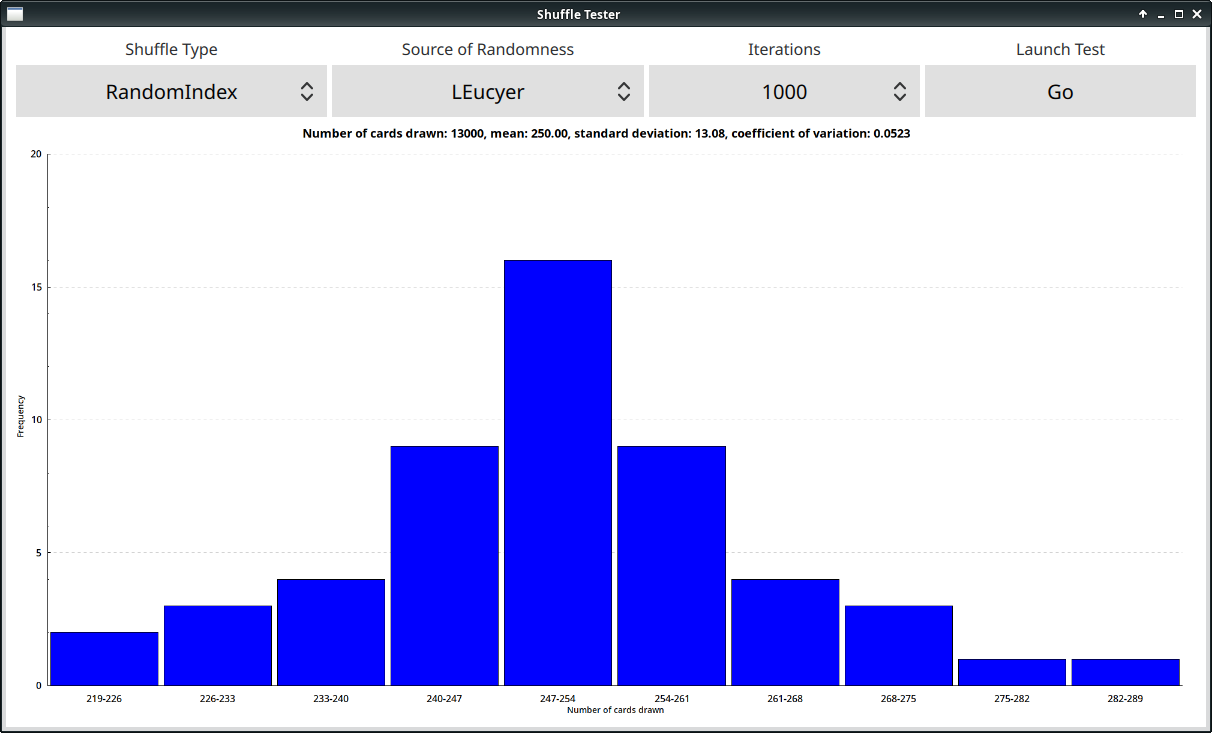
\includegraphics[width=\linewidth]{../images/shuffletester2.png}}
    \caption{The modified shuffle tester program}%
    \label{fig:shuffletester2}
\end{figure}

As you can see, the chart follows a typical normal distribution. Most cards are
picked an average amount, with a few cards being picked a lesser amount or
a greater amount. This gives us an easier way to easily see by eye how spread
out the data set is - a uniform shuffle and random source will give a normal
distribution with a very small standard deviation.

\begin{table}[H]
    \centering
    \begin{tabular}{l l l l}
    \toprule
                & RandomIndex   & Knuth & RandomSort  \\
    \midrule
    LEucyer     & 0.0054        & 0.0049& 0.0059      \\ \addlinespace
    Mersenee    & 0.0053        & 0.0062& 0.0059      \\ \addlinespace
    MWC256      & 0.0051        & 0.0061& 0.0062      \\ \addlinespace
    \bottomrule
    \end{tabular}
    \caption{The average CV for each shuffle and random source after 100,000
             iterations}
\end{table}

As the above results show, there is not a massive amount of difference between
the CV of the shuffles. We see the RandomIndex algorithm gets consistently low
CV's, followed by the Knuth algorithm, with RandomSort producing the highest
CV. If we then look at the random sources, we see both MWC256 and Mersenne
with an equal average CV, whilst LEucyer is slightly lower. This is odd, due
to LEucyer having the smallest bit size and cycle length, and we would expect
it to be a less effective RNG source. However, all these results are relatively
close together, and depending on P values used, could be discarded as within
the margin of error.

Secondly, to evaluate gameplay effects of these shuffles, two AI's were used.
The first, was the control AI, and would simply call any bet. The second
was a more sophisticated, rule based AI\@. This AI attempts to evaluate the value
of its hand in relation to the cards on the table at any time, and bets
correspondingly. This AI was then run, using each of the algorithms and
random sources against the control AI, and the win percentage was recorded,
after 1000 trials of each.

\begin{table}[H]
    \centering
    \begin{tabular}{l l l l}
    \toprule
                & RandomIndex   & Knuth & RandomSort  \\
    \midrule
    LEucyer     & 87.8\%        & 89.8\%& 90.4\%      \\ \addlinespace
    Mersenee    & 89.0\%        & 89.0\%& 88.1\%      \\ \addlinespace
    MWC256      & 90.1\%        & 89.7\%& 89.6\%      \\ \addlinespace
    \bottomrule
    \end{tabular}
    \caption{The win percentage of the rule-based-ai against the control
             call-any AI for each shuffle and random source}
\end{table}

As we can see, changing the shuffle type or random source doesn't appear to
effect the outcome very heavily, which is to be expected - even if the cards
were drawn in a slightly different way, we would see both players getting
altered cards, and so the effect would be mitigated. What we can see from this
data however, is that the rule based AI is relatively effective, winning on
average 89 games out of 100. Whilst the opponent it is playing against is very
trivial, this is sufficient to show that the AI is playing in a sane way, and
is very successful against weak opponents. In the future, it could be beneficial
to test the rule based AI against a large number of human opponents, to see
how effective it is in a real world scenario.

Finally, if the poker server is launched with a flag, the shuffle and random
source can be changed mid game, to see the live effect. Any updates to the
shuffle and random source only apply once the current round is finished, to
prevent corrupting the internal state of the card deck.

%%%%%%%%%%%%%%%%%%%%%%
\subsection{UI Design}
%%%%%%%%%%%%%%%%%%%%%%
Designing the graphical interface began with simple mockups. A simple
initial diagram is shown below.

\begin{figure}[h]
    \frame{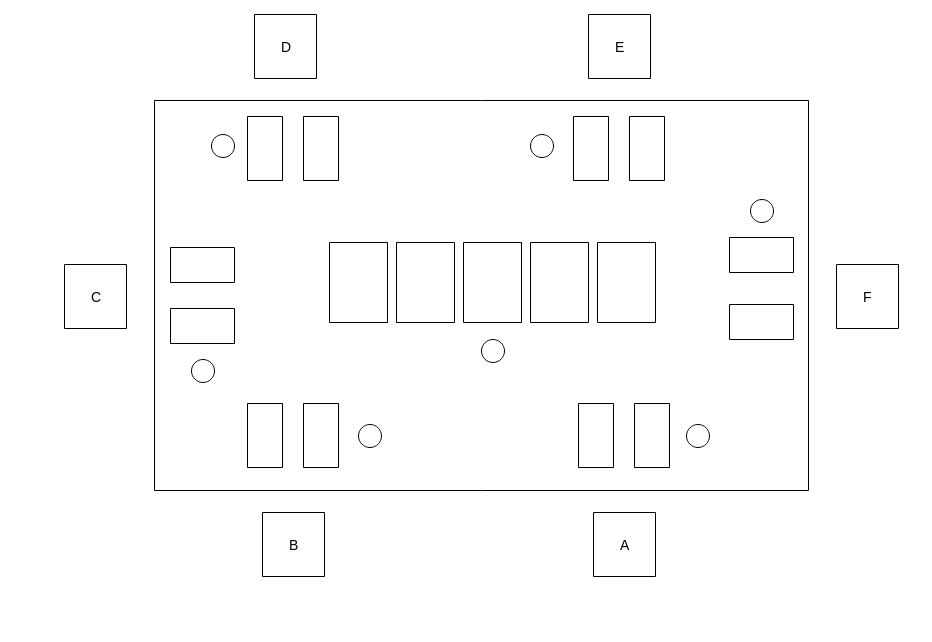
\includegraphics[width=\linewidth]{../images/initialgui.png}}
    \caption{Initial GUI mockup}%
    \label{fig:initialgui}
\end{figure}

This is a very standard design which cannot be varied much. All players have
two cards, a current bet, and a total amount of chips. As you may notice
in Figure~\ref{fig:initialgui} there is no label for the players total amount
of chips. This was instead decided to be stored as part of the name component,
as it makes for much less visual noise. The player labelled `A', is the
users player. He/she will always be seated here, and the other players will
be rotated around the board from their perspective. That is, every single
player A through F will appear to be in seat A from their own point of view.
The GUI is player centric. The relative positions, however will not be 
modified. Player A will always have player B to their left and Player F to 
their right, no matter where they visually appear to be. Of course, this has 
been implemented to not affect how the gameplay works, as the ordering of 
players is maintained, it is simply the visual representation of the players 
which is being manipulated.

The players need some way to interact with the game, and simple buttons which 
lie under the poker table were used for this. The raise button brought some 
complications, as the user has to enter a valid integer to increase the current
bet to. Some constraints are placed on this parameter.

\begin{itemize}
\item The user must have enough chips to make the raise
\item The user must raise by at least the minimum raise
\item The raise must be an integer, not fractional
\end{itemize}

It was decided to use a separate window with a slider to handle the above
reasons. A slider has a minimum, and a maximum. This prevents the user from
both raising too little, and too much. And, by setting a slide interval, it
prevents the user selecting a non integer.

\begin{figure}[h]
    \centering
    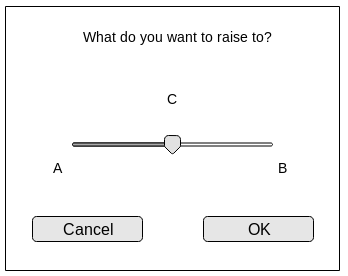
\includegraphics[width=0.5\linewidth]{../images/raisewindow.png}
    \caption{The Raise Window, where A is the minimum raise, B is the maximum
             raise, and C is the currently selected raise value}%
    \label{fig:raisewindow}
\end{figure}

However, in the implementation of this, it was found that when displaying
the selected value, despite the steps being integer steps of one, 
fractional values could arise due to inherent errors in floating point 
mathematics. This was solved by simply taking the raw slider value, and 
casting it to an integer variable. This variable was then used for displaying 
the current users selection, and for the program to take as the chosen value 
once the `OK' button had been selected. Figure~\ref{fig:raisewindow} shows the 
raise window, where A is the minimum value, B is the maximum value, and C is 
the current value. It should be noted that these values are denoted in chips,
and no particular currency is implied, though most casinos usually peg a
fiat value to a chip.

\begin{figure}[H]
    \centering
    \begin{subfigure}[h]{0.4\textwidth}
        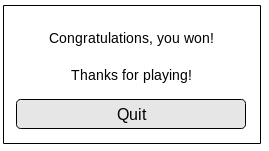
\includegraphics[width=\textwidth]{../images/winscreen.png}
        \caption{The Win Window}%
        \label{fig:winwindow}
    \end{subfigure}
    \begin{subfigure}[h]{0.4\textwidth}
        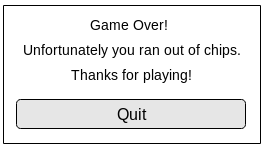
\includegraphics[width=\textwidth]{../images/lossscreen.png}
        \caption{The Loss Window}%
        \label{fig:losswindow}
    \end{subfigure}
    \caption{The Game Over Windows}\label{fig:gameoverwindows}
\end{figure}

Finally, there were elements needed for when a player either wins the game,
by the other players being eliminated for running out of chips, or when a
player loses, by being eliminated themselves. These took the form of simple
windows with configurable text, and a quit button. Both the win window
and the loss window use the same component, with only differing text. This
keeps the GUI consistent, and thus increases user acceptance.

Once the mockups had been completed the GUI was implemented in QtQML,
and hooked up to the Haskell code so it was fully usable and could be used
to test the poker game. Figure~\ref{fig:actualgui} shows the GUI in use,
with 6 players participating in a game. 

\begin{figure}[H]
    \centering
    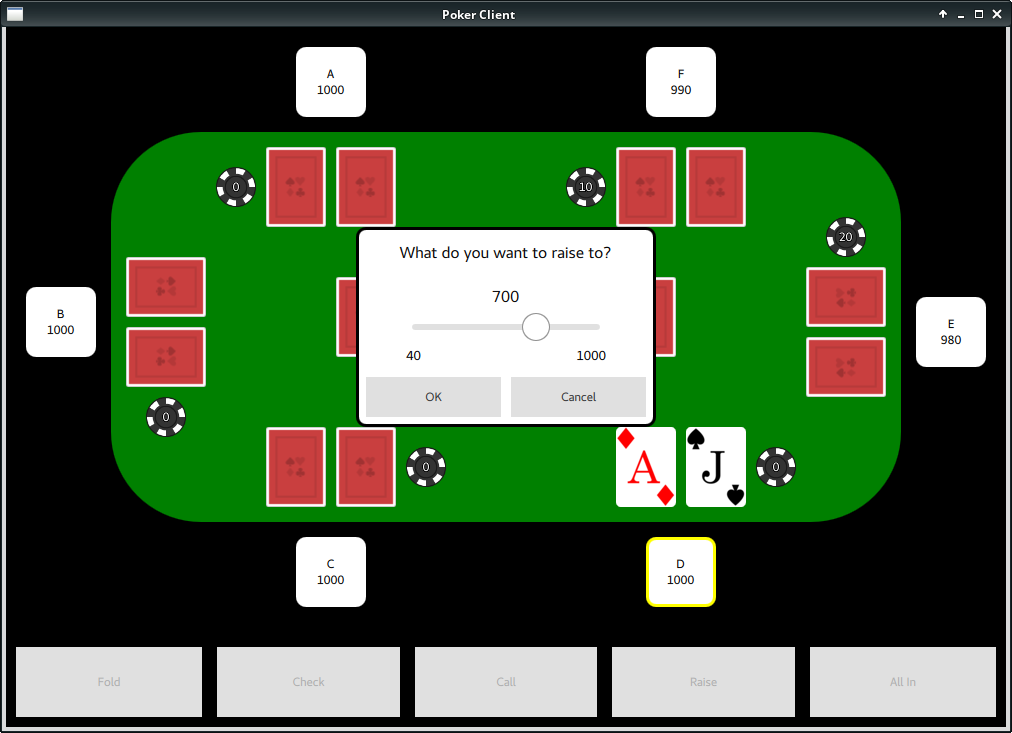
\includegraphics[width=\textwidth]{../images/actualgui.png}
    \caption{The initial implemented GUI}%
    \label{fig:actualgui}
\end{figure}

You can also see the implemented raise window in this image. Aside from the 
obvious card and poker chip assets, and colours, the implemented GUI is 
essentially the same as the mockup. One difference that was decided upon 
adding whilst testing, was a yellow border around the current player, so users 
would know how long it was until it was their turn. 

One feature of note is button fading. When buttons are unavailable, for
example if it's not the players turn, or a certain action would be invalid,
the buttons are greyed out, and unclickable. When actions become available,
they are clickable and fully coloured. This is an easy way to let players
know the valid actions whilst keeping the GUI consistent. Faded and non faded
buttons can be seen in figure~\ref{fig:guiwithconsole}.

Another modification considered making was adding a dealer chip. Whilst
online poker does not have an actual player who deals the cards, and indeed
in real life poker the dealer is often not an actual player, the concept of
a dealer is still used.

Each round, the dealer progresses, and the player to
the left of the dealer is the player who bets first. In the preflop, this
player has to play a forced blind, but once in the flop and beyond, this player
gets to bet first, which is of some strategic importance. 

For these reasons, a dealer chip would seem obvious, however it was decided
against, because it both clutters the GUI, and the dealer can still be
recognised by simply observing who plays the small blind, and retaining this
information, knowing the dealer progresses once to the left each full round.
In the above screenshot for example, the dealer can be identified to be A,
as the player to his left has played a small blind of 10 chips.

One modification that was added after the initial implementation was a text
console. This was used because some important information was difficult to 
display graphically, had to be interpreted very quickly, or was useful to be 
consulted at a later point in the game. The text console allowed messages such 
as bet history and hand values to be constantly visible to allow players to 
digest at their own pace.

\begin{figure}[H]
    \centering
    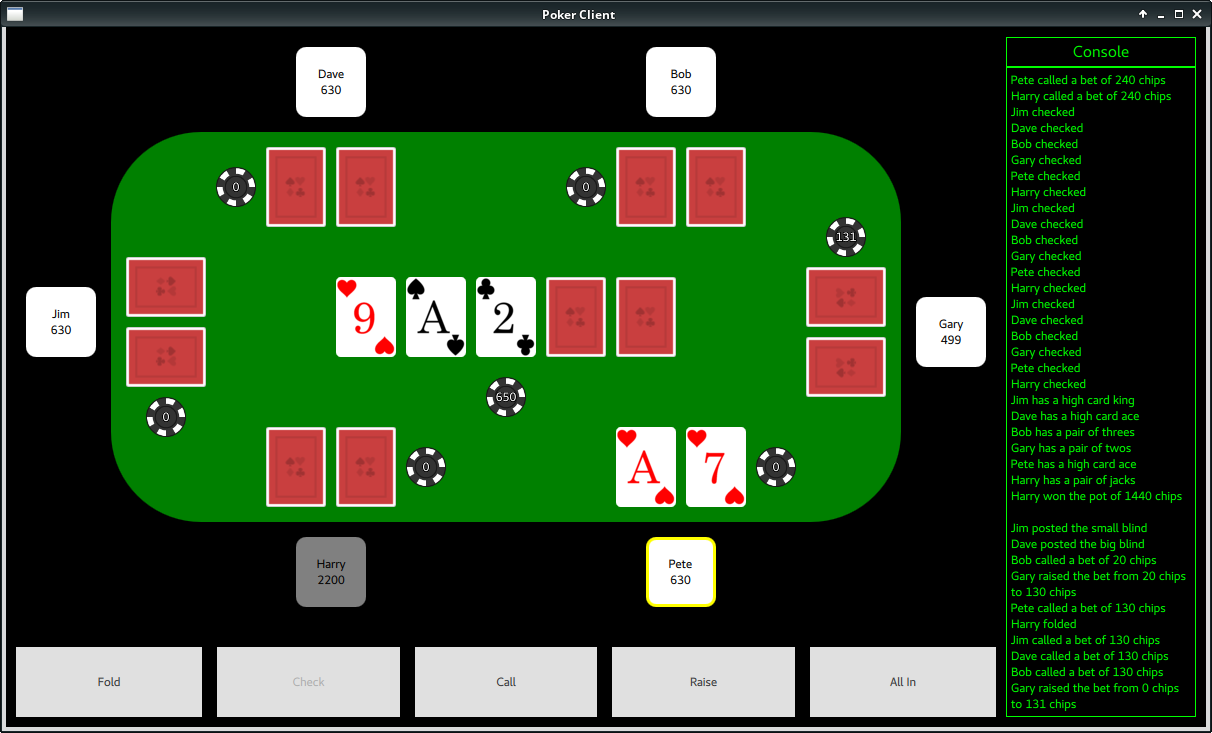
\includegraphics[width=\textwidth]{../images/guiwithconsole.png}
    \caption{The GUI with text console}%
    \label{fig:guiwithconsole}
\end{figure}

\newpage{}

%%%%%%%%%%%%%%%%%%%%%%%%%%
\subsection{System design}
%%%%%%%%%%%%%%%%%%%%%%%%%%

Not sure what should go here yet.

\newpage{}

%%%%%%%%%%%%%%%%%%%%%%%%%%%%%%%%%%%%%%%%%%%%%%%%%
\subsection{System Implementation of Simple AI's}
%%%%%%%%%%%%%%%%%%%%%%%%%%%%%%%%%%%%%%%%%%%%%%%%%
Three simple AI's were developed during the development of the software system.
Firstly, an AI framework was created. This handled communication with the
server and startup, requiring an AI to only implemented one single function,
that returns the chosen action of the AI to the server. This function takes
as an argument an array of valid actions, so the AI doesn't have to determine
which actions are valid within the current context. This framework turned out
to be very advantageous later on, when some simple control AI's were wanted
to be implemented. Two of the three AI's developed are trivial to implement
and explain. The first, would simply choose one of the valid actions at
random and return it. In the case that it chose raising as the action, it
would raise a random amount between the minimum raise and the AI's total
balance.

Algorithm~\ref{code:randomai} describes this programs high level execution.

\vspace{0.3cm}

\begin{algorithm}[H]
    \SetKwInOut{Input}{input}\SetKwInOut{Output}{output}
    \Input{An array of valid actions $actions$}
    \Output{A single action $action$}
    \BlankLine{}
    \nlset{STEP 1} $randomNum \leftarrow getRandomNum(0, length(actions))$\;
    \nlset{STEP 2} $action \leftarrow actions[randomNum]$\;
    \nlset{STEP 3} \If{$action$ == $raise$}{
                        $action.raiseAmount \leftarrow getRandomNum(state.minimumRaise, player.balance)$\;
                   }
    \nlset{STEP 4} return $action$\;
\caption{Implementation of an AI that picks a random action}%
\label{code:randomai}
\end{algorithm}

\vspace{0.3cm}

We can see here the power of the AI framework, allowing a full client to connect
to the server, exchange messages with it, and be able to choose how to bet
in only four simple lines of code.

The second AI, the control AI, is even simpler. This AI simply matches every
bet, and is used to measure the other AI's performance in a percentage of
win rate. Algorithm~\ref{code:controlai} describes this programs high level
execution.

\vspace{0.3cm}

\begin{algorithm}[H]
    \SetKwInOut{Input}{input}\SetKwInOut{Output}{output}
    \Input{An array of valid actions $actions$}
    \Output{A single action $action$}
    \BlankLine{}
    \nlset{STEP 1} \If{$call$ \text{is member of} $actions$}{
                        return $call$\;
                   }
                   \If{$check$ \text{is member of} $actions$}{
                        return $check$\;
                   }
                   \If{$raise$ \text{is member of} $actions$}{
                        return $raise$\;
                   }
                   \Else{
                        return $allin$\;
                   }
\caption{Implementation of an control AI that always matches any bet}%
\label{code:controlai}
\end{algorithm}

\vspace{0.3cm}

Finally we have the rule based AI, which is relatively good at the game and
can beat amateur players at poker. This AI calculates the value of its hand
relative to the table's hand. For example, if there is a straight (Five cards
in a row) in the community cards, that is a powerful hand, but because it
is from the community cards, everyone else also has that hand. Hence, we need
to calculate how strong the AI's cards are in unison with the community cards.
The AI then simply alters the amount it is willing to bet or call based on the
calculated value of the hand. It will bet larger amounts with better hands,
and if its hand is weak, it will fold when the bet is raised. Due to this
simplistic approach to the game, it reveals a large amount of information
about its hand based on it's bets. If the AI consistently bets large amounts,
it has a strong hand from the beginning. If it bets nothing initially then
starts betting after a card is revealed, it is easy for the other players to
narrow down what possible hands they have. To improve this, the AI could
make occasional bluffs. Another mitigation would be to have set bet sizes,
for example a small, medium, and large bet size where the nearest one is rounded
to when the value is calculated. This causes less information to be leaked
about the strength of the AI's hand when they bet. Finally, if a large increase
in the value of the hand is detected, the AI could lower their bet to the smaller
bet size and ramp up the bet size as the rounds go on. This prevents revealing
that the AI's hand value has suddenly increased.
Algorithm~\ref{code:rule-based-ai} describes this programs high level execution.

\vspace{0.3cm}

\begin{algorithm}[H]
    \SetKwInOut{Input}{input}\SetKwInOut{Output}{output}
    \Input{An array of valid actions $actions$}
    \Output{A single action $action$}
    \BlankLine{}
    \nlset{STEP 1} $evAllCards \leftarrow evaluateCards(player.cards + state.cards)$\;
    \nlset{STEP 2} $evCommunityCards \leftarrow evaluateCards(state.cards)$\;
    \nlset{STEP 3} $betSize \leftarrow evAllCards - evCommunityCards$\;
    \nlset{STEP 4} \If{$betSize$ $<$ 0 \&\& $check$ \text{is member of} $actions$}{
                        return $check$\;
                   }
                   \If{$betSize$ $<$ 0}{
                        return $fold$\;
                   }
                   \If{$betSize$ $>=$ $state.minimumRaise$ + $state.currentBet$ \&\& $player.balance$ $>=$ $betSize$}{
                        return $raise(betSize)$\;
                   }
                   \If{$betSize$ $>=$ $state.bigblind$ $*$ 100} {
                        return $allin$\;
                   }
                   \If{$betSize$ $>=$ $state.currentBet$ \&\& $check$ \text{is member of} $actions$}{
                        return $check$\;
                   }
                   \If{$betSize$ $>=$ $state.currentBet$ \&\& $player.balance$ $>=$ $betSize$}{
                        return $call$\;
                   }
                   \If{$check$ \text{is member of} $actions$}{
                        return $check$\;
                   }
                   \Else{
                        return $fold$\;
                   }
\caption{Implementation of a rule based AI}%
\label{code:rule-based-ai}
\end{algorithm}

\vspace{0.3cm}

As you can see, the AI is relatively simple and is just based off a few rules.
All the AI does is choose the most optimal action based of the target bet
value. For example, if the target bet is above the current bet and the AI
has enough chips, it should raise. If it doesn't have enough chips, it should
instead call. The code to calculate the target bet is taken from the
poker-eval \parencite{code:dachary2004} library, which was chosen to allow
AI's to be developed quickly. A similar library to this was developed to
evaluate a hand of cards in comparison to another hand of cards, for determining
who has the strong hand, however this only creates an order, and not a
numerical value determining the relative strength of a hand.

%%%%%%%%%%%%%%%%%%%%%%%%%%%%%%%%%%%%%%%%%%%%%%%%%%%%%%%%%%%%%%
\subsection{System Implementation of Randomness and Shuffling}
%%%%%%%%%%%%%%%%%%%%%%%%%%%%%%%%%%%%%%%%%%%%%%%%%%%%%%%%%%%%%%
In the game of poker, the house does not wager against players. In each
poker hand, a player always wins, unlike other popular casino games, such as 
blackjack or roulette. Instead the usual method for online poker companies and
indeed poker tables in real life to make money is the rake. The rake is the 
commission fee that a casino takes from players in some method, as their way 
of generating revenue.

The implementation of the rake varies between casinos and online poker
software. Some common ones are in the below table.

\begin{center}
    \begin{tabular}{l l}
    \toprule
    Mechanism           & Description                                               \\
    \midrule
    Pot Rake            & Percentage taken from the pot, per hand or betting round  \\ \addlinespace
    Dead Drop           & Fee paid by the player with the dealer button each hand   \\ \addlinespace
    Timed Rake          & Set fee collected every set interval of time              \\ \addlinespace
    Fixed Fee           & Fixed fee per hand                                        \\ \addlinespace
    Tournament Fee      & Entry fee to participate in poker tournaments             \\ \addlinespace
    Subscription Fees   & Players are charged a subscription fee to play            \\
    \bottomrule
    \end{tabular}
\end{center}

Finally, some games are rake free, instead generating revenue by driving
traffic to more profitable businesses. The software developed that this paper
is discussing is also rake free, due to being only for academic purposes.

However, despite companies being able to generate revenue in these ways, the
implementation of random number generation in poker software is a topic of
some interest. Possible issues include rogue employees writing malicious
code to give them or people connected to them beneficial cards, faulty code
allowing the random number generation to be exploited, and other schemes, such
as giving newer players or failing players better cards, to encourage them to 
continue using the companies platform, and generating revenue through rakes.

For these reasons, random number generation has been analysed and multiple
different shuffling algorithms or card picking algorithms have been
developed and contrasted for possible weaknesses. Two obvious approaches to 
selecting cards are:

\begin{itemize}
    \item Storing an array of all the cards and indexing this array in some way to take a card
    \item Shuffling an array in some way and taking the top item
\end{itemize}

It was hypothesised that the random number implementation and card picking
algorithms could effect the cards generated, and potentially lead to a more
predictable, non random game. For this reason, multiple algorithms and
different sources of randomness has been developed and tested, along with two
complementary programs to test them. Firstly, a GUI which can be launched
when the `--chooseshuffle' argument is given to the server, allows the card
picking algorithm and random source to be altered mid game.

This program simply allows the user to change the shuffle and random source
by picking from a list. Once this item is changed, internally a variable is
assigned to the new chosen shuffle and random source, and upon the round
being completed, the method for drawing cards is updated with the new user
selected function. This prevents the method being changed mid round, which
has a high potentially to cause bugs, due to the deck state having to be
maintained. Upon subsequent rounds, the new chosen functions will be used
to draw cards.

\begin{figure}[H]
    \centering
    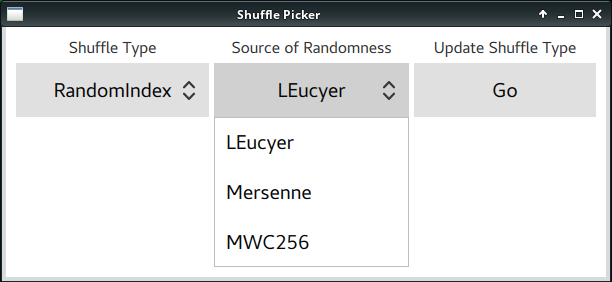
\includegraphics[width=0.8\linewidth]{../images/shufflepicker.png}
    \caption{The Shuffle Picker Window}%
    \label{fig:shufflepicker}
\end{figure}

Another program provides a similar interface but instead allows multiple hands 
to be drawn and the number of times each card was drawn displayed in a graph. 
This allows us to easily see the effect of the different algorithms on the 
uniformness of the card distribution. Each iteration draws 17 cards from
a new deck. This number is chosen because in this implementation of the game,
the maximum number of players is 6, and there are 5 cards displayed on the
table. Hence, with 2 cards each, $2 * 6 + 5 = 17$. As each card is drawn,
it is added to a card dictionary. If the card already exists, the number seen
of this card is incremented. If not, the card is inserted, with an initial
value of 1. 

\begin{figure}[H]
    \centering
    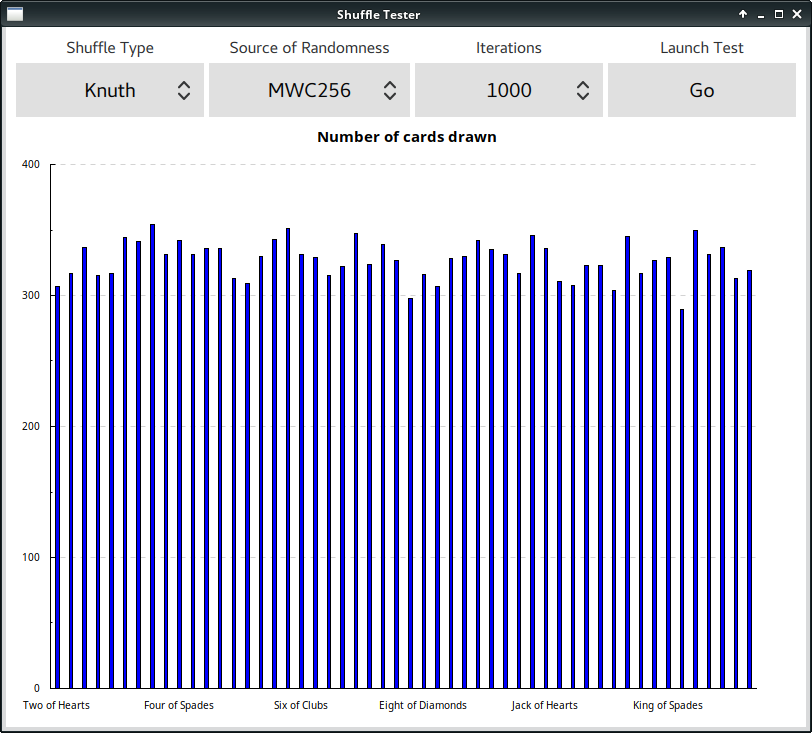
\includegraphics[width=0.8\linewidth]{../images/shuffletester.png}
    \caption{The Shuffle Tester Program}%
    \label{fig:shuffletester}
\end{figure}

Algorithm~\ref{code:shuffletester} describes this programs high
level execution.

\vspace{0.3cm}

\begin{algorithm}[H]
    \nlset{STEP 1} launch GUI\;
    \While{close button not pressed}{
        \If{go button pressed}{
            \nlset{STEP 2} $iterations \leftarrow \text{selected number of iterations}$\;
            $drawFunction \leftarrow \text{selected card draw function}$\;
            $randomSource \leftarrow \text{selected source of randomness}$\;
            $cardMapping \leftarrow []$\;
            \nlset{STEP 3} \For{$i \leftarrow 0$ \KwTo{} $iterations$}{
                $deck \leftarrow \text{new deck}$\;
                $cards \leftarrow []$\;
                \For{$j \leftarrow 0$ \KwTo{} $17$}{
                    \nlset{STEP 4} $card \leftarrow drawCard(drawFunction, randomSource, deck)$\;
                    \If{$card$ \text{is member of} $cardMapping$}{
                        cardMapping[card]++\;
                    }
                    \Else{
                        insert ($cardMapping$, $card$, 1)\;
                    }
                }
            }
            \nlset{STEP 5} $barChart \leftarrow []$\;
            \nlset{STEP 6} \For{$i \leftarrow 0$ \KwTo{} length ($cardMapping$)}{
                createBar ($barChart$, $cardMapping[i]$)\;
            }
            \nlset{STEP 7} display ($barChart$)\;
        }
    }
\caption{The shuffle tester algorithm}%
\label{code:shuffletester}
\end{algorithm}

\vspace{0.3cm}

The three sources of randomness used are:

\begin{itemize}
    \item Portable Combined Generator of L'Eucyer \parencite{leucyer1988}
    \item Faster Mersenne Twister \parencite{matsumoto1998,saito2008}
    \item Multiply With Carry 256 \parencite{marsaglia2003}
\end{itemize}

\begin{center}
    \begin{tabular}{l l l}
    \toprule
    Random Source           & Bit Size  & Cycle Length  \\
    \midrule
    L'Eucyer                & 32        & $ \displaystyle \frac{(2147483563-1)(2147483399-1)}{2}$   \\ \addlinespace
    Fast Mersenne Twister   & 128       & $ \displaystyle {2}^{19927}-1$                            \\ \addlinespace
    Multiply With Carry 256  & 32        & $ \displaystyle {2}^{8222}$                               \\
    \bottomrule
    \end{tabular}
\end{center}

These cycle lengths are sufficiently long that it would be very difficult
for an attacker to use the knowledge of the period length to their advantage,
as even the algorithm with the lowest cycle (L'Eucyer's), allows for
approximately $1.35e17$ hands to be dealt before the generator cycle ends.

The bit size is not an issue in the RandomIndex and KnuthShuffle
implementation, as they only require random numbers to be equally distributed
between 0 and 51. However, RandomSort generates one random number for each
card, then sorts the card list based on the number generated. Therefore, if
the same number is generated more than once, the shuffle will be non random.
We can compute the probability of the same number being picked more than once
using equation~\ref{eq:probSameNumSimple}.

\begin{equation} \label{eq:probSameNumSimple}
\begin{split}
& k = 2^\text{bit size}\\
& p = 1 - \frac{k!}{{k^{52}}(k - 52)!}
\end{split}
\end{equation}

Factorials of the large numbers we are using are numerically complex to
calculate, so a simplification is shown in equation~\ref{eq:probSameNumFast}.

\begin{equation} \label{eq:probSameNumFast}
\begin{split}
& k = 2^\text{bit size}\\
& p = 1 - \frac{\displaystyle\prod_{i=0}^{51} k - i}{k^{52}}
\end{split}
\end{equation}\\

If we have a 32 bit number, $p = 3.08\num{e-7}$.\\
For a 128 bit number, $p = 3.89\num{e-36}$.\\

Therefore, the chance of the same number being picked more than once is small,
and so the shuffle has a high probability to be uniform.

Whilst testing the shuffles with the shuffle tester, it was discovered that
the Knuth shuffle with the Mersenne twister algorithm would deal cards in a
non uniform manner. As we can see in~\ref{fig:faultymersenne}, the first 17
cards in the deck were approximately 5\% less likely to be drawn.

\begin{figure}[H]
    \centering
    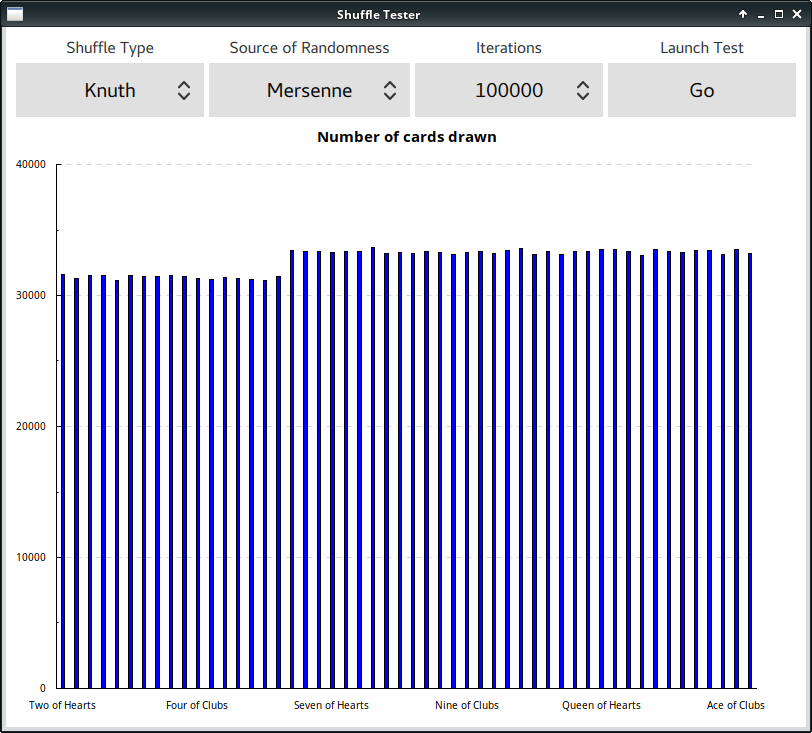
\includegraphics[width=0.8\linewidth]{../images/faultymersenne.png}
    \caption{The Non Uniform Mersenne Distribution}%
    \label{fig:faultymersenne}
\end{figure}

This was due to the random library having no function allowing random numbers
within a range to be generated, and instead a na\"{\i}ve implementation was
used, as in Algorithm~\ref{code:rngBadCapping}. In this version of
getRandomNumber, no bounds are given, and the function simply returns a
random number in the range of an integer.

\vspace{0.3cm}

\begin{algorithm}[H]
    \SetKwInOut{Input}{input}\SetKwInOut{Output}{output}
    \Input{An integer $maxValue$}
    \Output{A random number of maximum $maxValue$}
    \BlankLine{}
    \nlset{STEP 1} $x \leftarrow getRandomNumber$\;
    \nlset{STEP 2} return $x$ \% $maxValue$\;
\caption{Initial random number capping implementation}%
\label{code:rngBadCapping}
\end{algorithm}

\vspace{0.3cm}

Due to the the values not begin distributed evenly, this resulted in the
above non uniform distribution. This was solved by using an algorithm in which
all the possible values of the random number generator are divided into equal
sized intervals, each representing one of the desired values. For example
if the maximum number the random number generate can create is 11, and the
desired values are a range from 0 to 5, \{0,1\} would be assigned to 0, \{2,3\}
to 1, and so on. This new version can be seen in
Algorithm~\ref{code:rngGoodCapping} \parencite{website:reich2011}.

\vspace{0.3cm}

\begin{algorithm}[H]
    \SetKwInOut{Input}{input}\SetKwInOut{Output}{output}
    \Input{An integer $maxValue$}
    \Output{A random number of maximum $maxValue$}
    \BlankLine{}
    \nlset{STEP 1} $range \leftarrow 1 + maxValue$\;
    \nlset{STEP 2} $buckets \leftarrow {2}^{32}\; / \;range$\;
    \nlset{STEP 3} $limit \leftarrow buckets \times range$\;
    \nlset{STEP 4} $x \leftarrow 0$\;

    \nlset{STEP 5} \While{$x$ $<$ $limit$}{
        $x \leftarrow getRandomNumber$\;
    }

    \nlset{STEP 6} return $x$ / $buckets$\;
\caption{Revised random number capping implementation}%
\label{code:rngGoodCapping}
\end{algorithm}

\vspace{0.3cm}

To an extent this demonstrates how easy it would for poker software to have
biased distributions if rigorous testing procedures were not in place.

After implementing the above shuffle tester, and comparing the results,
it was concluded that all shuffles and sources of randomness appear at face
level to be sufficiently random, and not effected by the implementation chosen.
However, as early mentioned, it is very simple for an implementation to be
incorrectly developed, causing non random cards to appear.

A simple way for a malicious actor to generate cards which appear to be random
but actually benefit or hinder a player is to generate cards in a random
way, as in one of the above algorithms, then inspect the generated cards,
and distribute them to players in a specific way to cause the desired effect.
For example, if there were 3 players, and the generated cards were
[Ace, Ace, Seven, Seven, Two, Two], both the aces could be distributed to
the player who has the least chips, whilst the other two players both receive
a seven and two, the statistically worst hand in Texas Hold-Em Poker.

Using this method of rewarding the players with less chips, whilst the overall 
hands and cards generated will be uniform, the cards dealt to each player 
will not be. This could still be measured, but is harder to do so. If the
method is repeatedly applied, in that a player will gain chips by being dealt 
favourable hands and lose chips when dealt bad hands, the player would have 
a cycle of good to bad cards dealt to him as his chips decrease and increase, 
and so might be difficult to detect over long periods, as the highs and lows 
would cancel out.

However, this would be possible to detect if a player is particularly good, or
particularly bad. If they are particularly good, and play their bad hands well
to minimise their chip loss, they will over long periods have a non uniform
card distribution due to constantly having more chips than the average player.

Again, this can be mitigated by dealing uniformly distributed cards to all
players, but instead manipulating the table cards, so flops which benefit
the players with less chips' hands. In this way, a good player still receives
the amount of AA hands as a poorer player, but upon having this AA hand will
find that other players achieve three of a kinds, two pairs, flushes etc
with their lower ranked hands.

Software with rigged gameplay has been observed in the wild too. In 2011 
`BLR Technologies' was discovered to have been utilising rigged odds, with an 
observed win rate of $24.70\%$ compared to an expected win rate of $49.29\%$,
after having played 328 rounds. The chance of this occurring is 1 in 
146,107,962. \parencite{website:shackleford2011} After these allegations, 
the companies software was dropped by a casino software aggregator, `5Dimes'.

In conclusion, whilst we can demonstrate random number generation algorithms
to be hard or impossible to manipulate by the end user, the creator can do so
in harder and harder to detect ways to the casino's benefit. It is for this
reason that casinos must be transparent about their algorithms and allow
for rigorous investigation by standards agencies.
